\begin{figure}[h]
    \centering
    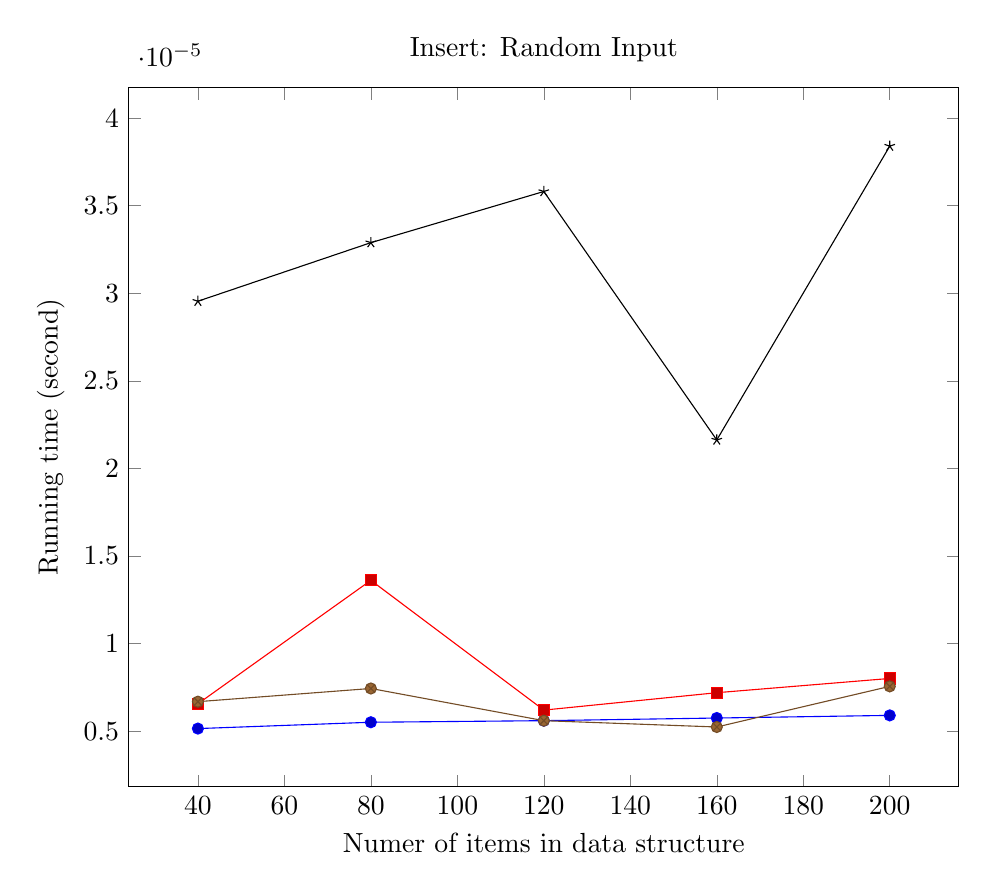
\begin{tikzpicture}
        \begin{axis}[
            xlabel={Numer of items in data structure},
            ylabel={Running time (second)},
            title={Insert: Random Input},
            width=\textwidth
        ]
		\addplot coordinates {
			(40, 5.150098258455138e-06)
			(80, 5.511508662553455e-06)
			(120, 5.601861263582197e-06)
			(160, 5.752448931956033e-06)
			(200, 5.903036600335421e-06)
		};
		\addplot coordinates {
			(40, 6.56562234118696e-06)
			(80, 1.3613125221179078e-05)
			(120, 6.204211937088644e-06)
			(160, 7.198090548365954e-06)
			(200, 8.011263957591331e-06)
		};
		\addplot coordinates {
			(40, 6.68609247588825e-06)
			(80, 7.439030817762982e-06)
			(120, 5.601861263582197e-06)
			(160, 5.2404508594783294e-06)
			(200, 7.559500952469822e-06)
		};
		\addplot coordinates {
			(40, 2.9545300535338548e-05)
			(80, 3.28883467732799e-05)
			(120, 3.5809747539777836e-05)
			(160, 2.162438917877041e-05)
			(200, 3.83998554358389e-05)
		};
        \legend{}
        \end{axis}
    \end{tikzpicture}
    \caption{Average of 0 operations, benchmarked every 0, starting at 0.}
\end{figure}